\chapter{STRATÉGIE MARKETING \& ACQUISITION RENFORCÉE}

\section{Programme "Building in Public"}

RBK 2.0 ne fait pas de publicité, elle produit de la preuve. Notre stratégie d'acquisition repose sur le "Building in Public". Nous documentons publiquement nos succès, nos échecs, nos audits et nos outils.
Cette transparence radicale a trois objectifs :
1. \textbf{Crédibilité :} Montrer le niveau technique réel avant même l'inscription.
2. \textbf{Confiance :} Rassurer les candidats (et leurs parents) sur le sérieux de la pédagogie.
3. \textbf{Communauté :} Attirer des mentors et des entreprises qui partagent nos valeurs.

\paragraph{Les 3 Piliers de Contenu}
\begin{enumerate}
    \item \textbf{Technique (The Code) :} Partage de snippets Rust, analyses de hacks récents, tutoriels Solana. Cible : Développeurs, CTOs.
    \item \textbf{Pédagogie (The Journey) :} Avant/Après des étudiants, rediffusion de Code Reviews, partage de ressources (Cheat Sheets). Cible : Candidats.
    \item \textbf{Success Stories (The Result) :} Interviews d'Alumni, montants des bounties gagnés, projets lancés. Cible : Grand public.
\end{enumerate}

\begin{figure}[H]
    \centering
    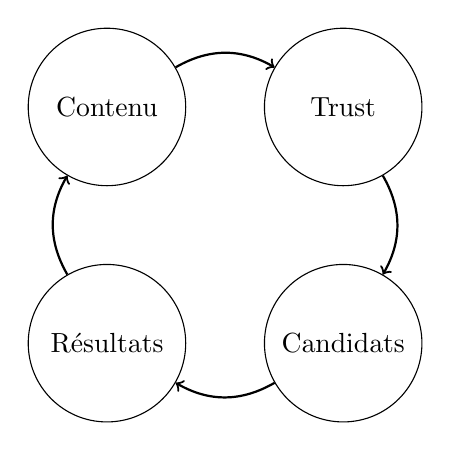
\begin{tikzpicture}
        \node[circle, draw, minimum size=2cm] (content) {Contenu};
        \node[circle, draw, minimum size=2cm, right of=content, node distance=3cm] (community) {Trust};
        \node[circle, draw, minimum size=2cm, below of=community, node distance=3cm] (apply) {Candidats};
        \node[circle, draw, minimum size=2cm, left of=apply, node distance=3cm] (result) {Résultats};
        
        \draw[->, thick, bend left] (content) to (community);
        \draw[->, thick, bend left] (community) to (apply);
        \draw[->, thick, bend left] (apply) to (result);
        \draw[->, thick, bend left] (result) to (content);
    \end{tikzpicture}
    \caption{Flywheel Building in Public}
\end{figure}

\begin{table}[H]
    \caption{Calendrier Éditorial Type (Cycle 12 Semaines)}
    \centering
    \small
    \rowcolors{2}{gray!10}{white}
    \begin{tabularx}{\textwidth}{|l|l|l|X|}
        \hline
        \textbf{Semaine} & \textbf{Thème} & \textbf{Canal} & \textbf{KPI Cible} \\ \hline
        S1-S4 & Rust Tips \& Tricks & Twitter/X & 10k Impressions \\ \hline
        S5-S8 & Démo Projets Élèves & YouTube/LinkedIn & 50 Leads (Inscrits Webinar) \\ \hline
        S9-S12 & Audit \& Sécurité & Blog/Medium & 5 Partenariats Entreprise \\ \hline
    \end{tabularx}
\end{table}

\section{Simulateur de ROI Interactif}

Pour contrer l'objection du prix, nous proposons un outil permettant de comparer 3 scénarios d'investissement. L'objectif est de montrer que le risque est nul si on commence petit.

\paragraph{Les 3 Options du Simulateur}
\begin{enumerate}
    \item \textbf{Option A (Prudent) :} Niveau 1 seul (2 900 TND). Objectif : Tester son appétence. Risque minime.
    \item \textbf{Option B (Standard) :} Niveau 1 + Upgrade Bundle. Coût total $\approx$ 14 900 TND. Objectif : Flexibilité.
    \item \textbf{Option C (Engagé) :} Bundle Upfront (14 900 TND). Objectif : Économie maximale immédiate.
\end{enumerate}

\begin{center}
\fbox{\begin{minipage}{0.9\textwidth}
\textbf{Exemple Chiffré : Le "Smart Start"} \\
\textit{Profil :} Étudiant, hésitant. \\
\textit{Action :} S'inscrit au \textbf{Niveau 1} (2 900 TND). \\
\textit{Résultat :} Valide ses acquis en 8 semaines. Réalise un premier Bounty de 500\$. \\
\textit{Décision :} Réinvestit le bounty dans l'upgrade Bundle. \\
\textbf{ROI :} Il a financé 50\% de son N1 par le code avant même de finir.
\end{minipage}}
\end{center}

\begin{table}[H]
    \caption{ROI Comparatif par Option (Sortie Junior : 3 000 TND/mois)}
    \centering
    \small
    \rowcolors{2}{gray!5}{white}
    \begin{tabularx}{\textwidth}{|l|l|l|X|}
        \hline
        \textbf{Option} & \textbf{Coût Total} & \textbf{Délai ROI} & \textbf{Avantage} \\ \hline
        N1 Seul & 2 900 TND & 1 mois & Test Low-cost \\ \hline
        Bundle & 14 900 TND & 5 mois & Accès complet + Job \\ \hline
        ISA & 15\% Salaire & Dès 1er salaire & Pas de cash upfront \\ \hline
    \end{tabularx}
\end{table}

\section{Stratégie Multi-Canaux}

Nous ne cherchons pas à être partout, mais à dominer 5 canaux spécifiques où se trouve notre cible "Elite".

\paragraph{Les 5 Canaux Prioritaires}
\begin{enumerate}
    \item \textbf{LinkedIn (La Vitrine) :} Pour les parents, les recruteurs et les partenariats corporatifs. \textit{Cadence : 2 posts/semaine.}
    \item \textbf{X / Twitter (L'Arène) :} Pour la crédibilité technique crypto, les news Rust, et l'engagement communautaire. \textit{Cadence : Quotidien.}
    \item \textbf{YouTube (La Preuve) :} Replays de workshops, Démos de Capstones, Témoignages. \textit{Cadence : 2 vidéos/mois.}
    \item \textbf{GitHub (Le CV) :} C'est notre canal d'acquisition "silencieux". Des repos propres et étoilés attirent les curieux techniques.
    \item \textbf{Discord (Le Salon) :} Conversion des leads chauds, support, Q\&A avant inscription.
\end{enumerate}

\begin{figure}[H]
    \centering
    \begin{tikzpicture}
        \node[draw] (aware) {Awareness (X/LinkedIn)};
        \node[draw, below of=aware] (consider) {Considération (YouTube/Webinar)};
        \node[draw, below of=consider] (intent) {Intention (Discord/Simulateur)};
        \node[draw, below of=intent, thick, fill=SolanaGreen!20] (action) {Action (Candidature)};
        
        \draw[->] (aware) -- (consider);
        \draw[->] (consider) -- (intent);
        \draw[->] (intent) -- (action);
    \end{tikzpicture}
    \caption{Funnel d'Acquisition Simplifié}
\end{figure}

\section{Programme de Référence \& Bounties}

Le "Word of Mouth" est notre canal le plus rentable (CAC $\approx$ 0). Nous l'industrialisons.

\paragraph{Système de Parrainage (Referral)}
Tout Alumni ou Étudiant validé peut parrainer un candidat.
\begin{itemize}
    \item \textbf{Pour le Parrain :} 500 TND (Cash ou déduction ISA) versés APRÈS la validation de la Période d'Essai du filleul (Anti-fraude).
    \item \textbf{Pour le Filleul :} 5\% de réduction immédiate sur les frais Upfront.
\end{itemize}

\paragraph{Programme "Bug Bounties" Pédagogiques}
Nous payons (en crédits ou token réputation) pour l'amélioration du cursus.
\begin{itemize}
    \item Typo majeure dans le cours : 10 pts.
    \item Optimisation d'un exercice de code : 50 pts.
    \item Fix de sécurité sur l'infra école : 500 TND.
\end{itemize}
Cela crée une culture de "Contribution" dès le premier jour.

\begin{table}[H]
    \caption{Catalogue des Incentives}
    \centering
    \small
    \begin{tabularx}{\textwidth}{|l|l|l|X|}
        \hline
        \textbf{Mécanisme} & \textbf{Bénéficiaire} & \textbf{Récompense} & \textbf{Condition Anti-Fraude} \\ \hline
        Parrainage & Alumni & 500 TND & Filleul valide le SPRINT 1 (pas juste inscrit). \\ \hline
        Ambassadeur & Influenceur & 10\% Commission & Lien tracké + KYC obligatoire. \\ \hline
        Bounty Code & Étudiant & Goodies / Cash & Pull Request validée par le Lead Tech. \\ \hline
    \end{tabularx}
\end{table}
